\section{Lasso estimatoren} \label{sec:lasso_estimatoren}
\textit{Dette afsnit er skrevet udfra kapitel 2 i \citep{hastie}.}

\textit{The Least Absolute Shrinkage Selection Operator}, som forkortes lasso, blev introduceret i \citep{lasso}. 
\begin{defn}[Lasso]
Lasso finder løsningen til optimeringsproblemet
\begin{align}
\widehat{\tbeta}^\text{lasso} = \argmin_{\tbeta \in \R^p} \cbr{\sum_{i=1}^n \del{y_i - \sum_{j=1}^p x_{ij} \beta_j}^2}, \ \text{underlagt at } \sum_{j=1}^p \vert \beta_j \vert \leq t. \label{eq:2.3}
\end{align} 
\end{defn}
Betingelsen $\sum_{j=1}^p \vert \beta_j \vert \leq t$ kan skrives mere kompakt som en \(\ell_1\)-norm betingelse $\Vert \tbeta \Vert_1 \leq t$.
Værdien af \(t\) begrænser summen af de absolutte værdier af parameter estimaterne og kontrollerer kompleksiteten af modellen. 
En lav værdi af \(t\) vil begrænse antallet af parametre, hvilket fører til en sparse model, som tilpasser data mindre præcis, mens en høj værdi af \(t\) betyder flere parametre og tillader dermed, at modellen tilpasser data meget præcis.

Lasso problemet kan omskrives til et Lagrange problem
\begin{align}
\widehat{\tbeta}^\text{lasso} = \argmin_{\tbeta \in \R^p} \cbr{ \Vert \y - \X \tbeta \Vert_2^2 + \lambda \Vert \tbeta \Vert_1}, \label{eq:2.5}
\end{align}
hvor $\lambda \geq 0$ er en såkaldt strafparameter. 
Der er en en-til-en korrespondance mellem det betingede problem \eqref{eq:2.3} og Lagrange problemet \eqref{eq:2.5}. 
For hver værdi af \(t\) hvor \(\Vert \tbeta \Vert_1 \leq t\) er opfyldt, da findes en tilhørende værdi af $\lambda$ som giver den samme løsning for \eqref{eq:2.5}.
Omvendt gælder der, at løsningen $\widehat{\tbeta}_\lambda$ til \eqref{eq:2.5} løser grænseproblemet med $t=\Vert \widehat{\tbeta}_\lambda \Vert_1$.
Værdien af \(\lambda\) skal specificeres ved en ekstern procedure kaldet \textit{krydsvalidering}, som vil blive diskuteret i kapitel \ref{ch:metoder}.

I andre beskrivelser af lasso estimatoren kan en faktor indsættes foran summeringen \eqref{eq:2.3} eller den euklidiske norm \eqref{eq:2.5} givet ved \(\frac{1}{2n}\) eller \(\frac{1}{2}\).
%Dette gør ingen forskel i \eqref{eq:2.3} og svarer blot til en simpel reparametrisering af \(\lambda\) i \eqref{eq:2.5}.
%Dette gør værdierne for \(\lambda\) sammenlignelige for stikprøver af forskellige størrelse, som er brugbart i krydsvalidering.

\textit{Ridge regression} estimatoren findes udfra 
\begin{align} 
\widehat{\tbeta}^\text{ridge} = \argmin_{\tbeta \in \R^p} \cbr{\sum_{i=1}^n \del{y_i - \sum_{j=1}^p x_{ij} \beta_j}^2}, \ \text{underlagt at } \sum_{j=1}^p \beta_j^2 \leq t, \label{eq:2.7} 
\end{align} 
hvor betingelsen $\sum_{j=1}^p \beta_j^2 \leq t$ kan skrives mere kompakt som en \(\ell_2\)-norm betingelse $\Vert \tbeta \Vert_2^2 \leq t$.
Ridge regression problemet kan også omskrives til et Lagrange problem
\begin{align*}
\widehat{\tbeta}^\text{ridge} = \argmin_{\tbeta \in \R^p} \cbr{ \Vert \y - \X \tbeta \Vert_2^2 + \lambda \Vert \tbeta \Vert_2^2},
\end{align*}
hvor $\lambda \geq 0$.
\begin{defn}[Ridge regression]
Estimatoren for ridge regression er givet ved
\begin{align} 
\widehat{\tbeta}^\text{ridge} = \del{\X^T \X + \lambda \mathbf{I}_p}^{-1} \X^T \y. \label{eq:ridge_estimator}
\end{align} 
\end{defn}
Estimatoren findes ved at differentiere \(\del{\y - \X \tbeta}^T \del{\y - \X \tbeta} + \lambda \tbeta^T \tbeta\) mht $\tbeta$, sætte dette lig 0 og isolere for $\tbeta$.
Ridge regression tilføjer altså en positiv konstant $\lambda$ på diagonalen af $\X^T \X$, hvilket medfører, at \(\X^T \X + \lambda \mathbf{I}_p\) er invertibel, selvom $\X$ ikke har fuld rang. 
Dermed er en entydig løsning altid garanteret. 
%
\begin{exmp}
Lad os betragte data givet i tabel \ref{tab:diabetes} fra \citep{efron}.
Datasættet består af målinger på 442 diabetes patienter, hvor responsvariablen er et kvantitativ mål af sygdom progressionen et år efter sygdommen er konstateret og følgende 10 prædiktorer: 
\begin{itemize}
\item \texttt{age}: patientens alder
\item \texttt{sex}: patientens køn
\item \texttt{bmi}: body-mass index
\item \texttt{map}: gennemsnitlig blodtryk
\item Målinger af blodet:  \texttt{tc},  \texttt{ldl}, \texttt{hdl}, \texttt{tch}, \texttt{ltg} og \texttt{tglu}
\end{itemize}
%
\begin{table}[H] 
\centering 
\begin{tabular}{cccccccccccc} 
& \texttt{age} & \texttt{sex} & \texttt{bmi} & \texttt{bp} & \multicolumn{6}{c}{Serum measurements} & \texttt{Response} \\
\cline{6-11}
Patient & \(\x_1\) & \(\x_2\) & \(\x_3\) & \(\x_4\) & \(\x_5\) & \(\x_6\) & \(\x_7\) & \(\x_8\) & \(\x_9\) & \(\x_{10}\) & \(\y\) \\
\midrule
1 & 59 &  1 & 32.1 & 101 & 157 & 93.2 & 38 &  4 & 2.11 & 87 & 151 \\
2 & 48 &  0 & 21.6 & 87 & 183 & 103.2 & 70  & 3 & 1.69 & 69  & 75 \\
3 & 72 &  1 & 30.5 & 93 & 156 & 93.6 & 41  & 4 & 2.03 & 85 & 141 \\
4 & 24  & 0 & 25.3 & 84 & 198 & 131.4 & 40 &  5 & 2.12 & 89 & 206 \\
5 & 50  & 0 & 23.0 & 101 & 192 & 125.4 & 52 &  4 & 1.86 & 80 & 135 \\
6 & 23 &  0 & 22.6 & 89 & 139 & 64.8 & 61 &  2 & 1.82 & 68 &  97 \\
\vdots & \vdots & \vdots & \vdots & \vdots & \vdots & \vdots & \vdots & \vdots & \vdots & \vdots & \vdots \\
441 & 36  & 0 & 30.0 & 95.0 & 201 & 125.2 & 42 & 4.79 & 2.23 & 85 & 220 \\
442 & 36 & 0 & 19.6 & 71.0 & 250 & 133.2 & 97 & 3.00 & 2.00 & 92 &  57 \\ \bottomrule
\end{tabular}  
\caption{Diabetes data. 442 diabetes patienter måles på 10 variable, hvor responsvariablen måler sygdomsprogressionen et år efter sygsommen er konstateret.} \label{tab:diabetes} 
\end{table} 
%
Datasættet, som vi betegner diabetes data, er inkluderet for at underbygge teorien og vi vil løbende i rapporten referere til det.
\end{exmp}
%
På figur \ref{fig:diabetes_koef} illustreres koefficientstierne for henholdsvis lasso og ridge regression for diabetes data.
Heraf ses at lasso udfører variabeludvælgelse og mindsker koefficienterne, mens ridge regression blot mindsker koefficienterne.
%
\imgfigh{diabetes_lasso_ridge.pdf}{0.9}{Koefficientstierne for lasso og ridge regression som funktion af $\log \del{\lambda}$ for diabetes data.}{diabetes_koef}

Betingelsesområderne for lasso og ridge regression for \(p=2\) illustreres på figur \ref{fig:LassoRig}.
%
\begin{figure}[H]
\centering
\begin{minipage}{0.4\linewidth}
\scalebox{0.7}{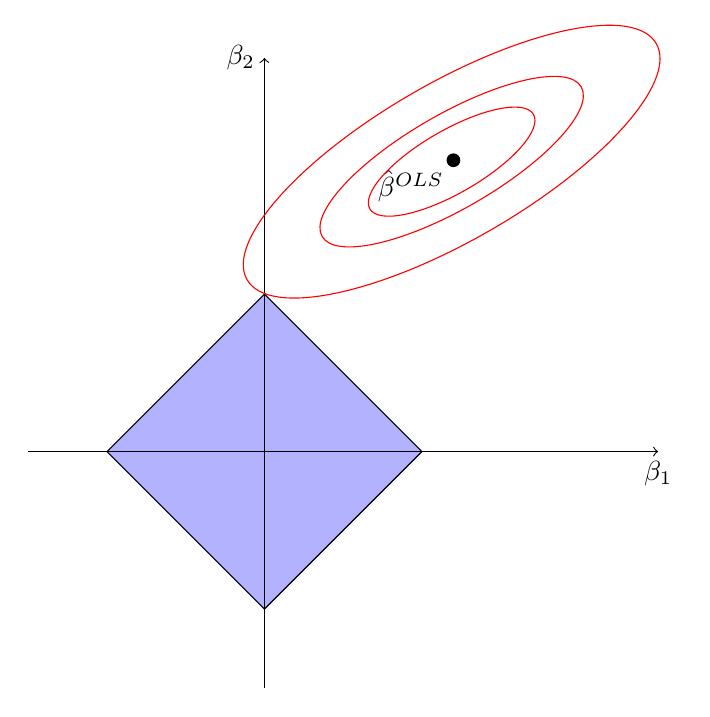
\begin{tikzpicture}
\draw [fill] (2.4,3.7) circle [radius=0.08];
\node [below left] (a) at (2.4,3.7) {$\hat{\beta}^\text{OLS}$};
\draw (-2,0) -- (0,2) -- (2,0)-- (0,-2) -- (-2,0)[fill = blue!30];
\draw [<-] (0,5) node [left] {$\beta_2$}-- (0,-3);
\draw[<-] (5,0) node [below] {$\beta_1$} -- (-3,0);
\begin{scope}[rotate = 30, red]
\clip[draw] (3.9,2) ellipse (3cm and 1cm);
\clip[draw] (3.9,2)ellipse (1.9 cm and 0.6 cm); 
\clip[draw] (3.9,2) ellipse (1.2 cm and 0.4 cm);
\end{scope}
\end{tikzpicture}}
\end{minipage}
\hspace{0.2cm}
\begin{minipage}{0.4\linewidth}
\scalebox{0.7}{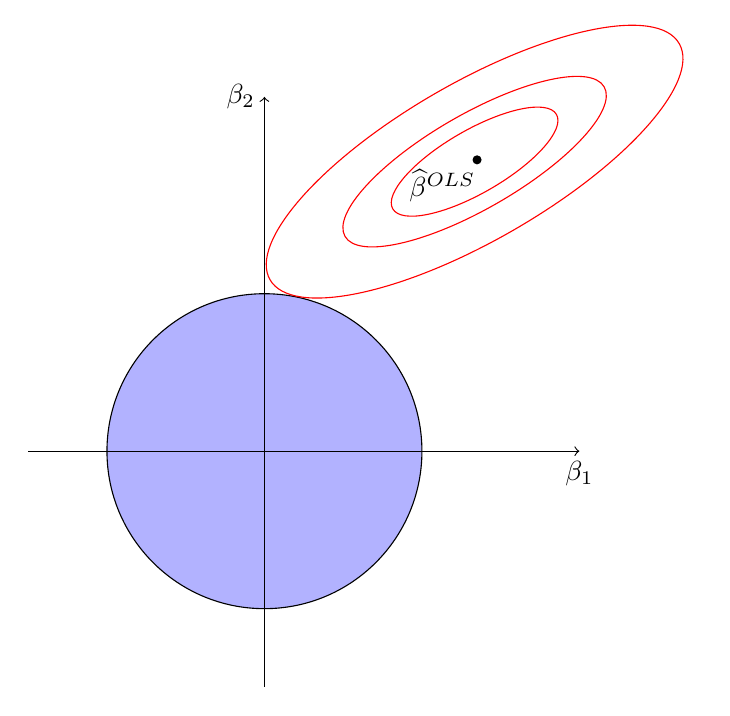
\begin{tikzpicture}
\draw [fill] (2.7,3.7) circle [radius=0.05];
\node [below left] (a) at (2.8,3.7) {$\widehat{\boldsymbol{\beta}}^\text{OLS}$};
\draw (0,0) circle (2cm) [fill= blue!30];
\draw [<-] (0,4.5) node [left] {$\beta_2$}-- (0,-3);
\draw[<-] (4,0) node [below] {$\beta_1$} -- (-3,0);
\begin{scope}[rotate = 30, red]
\clip[draw] (4.15,1.85) ellipse (3cm and 1cm);
\clip[draw] (4.15,1.85)ellipse (1.9 cm and 0.6 cm); 
\clip[draw] (4.15,1.85) ellipse (1.2 cm and 0.4 cm);
\end{scope}
\end{tikzpicture}}
\end{minipage}
\caption{Estimations illustration for lasso (venstre) og ridge regression (højre). 
De blå arealer er betingelsesområderne $\vert \beta_1 \vert+\vert \beta_2 \vert \leq t$ og $\beta_1^2+\beta_2^2 \leq t^2$, mens de røde ellipser er konturkurver for SSR. Konturkurverne har centrum i OLS estimatoren, $\widehat{\tbeta}^\text{OLS}$.} \label{fig:LassoRig}
\end{figure}
%
For $p=2$ er betingelsesområdet for lasso givet ved $\vert \beta_1 \vert + \vert \beta_2 \vert \leq t$, mens det for ridge regression er givet ved $\beta_1^2 + \beta_2^2 \leq t^2$.
Ellipserne omkring $\widehat{\tbeta}^{\text{OLS}}$ er konturkurverne for SSR, dvs. SSR er konstant i en given ellipse. Værdien af SSR stiger, som ellipsen udvides fra $\widehat{\tbeta}^{\text{OLS}}$.
Løsningen for lasso og ridge regression er givet ved det første punkt, hvor konturkurverne rammer betingelsesområderne.
Lasso har et regulært betingelsesområde, hvilket betyder, at hvis løsningen forekommer i et hjørne, da vil en af parametrene $\beta_j$ være lig 0.
Omvendt har ridge regression et cirkulært betingelsesområde, og derfor vil skæringen med konturkurverne generelt ikke være direkte på en akse.
Hvis $t$ er tilstrækkelig stor, da vil betingelsesområderne indeholde $\widehat{\tbeta}^{\text{OLS}}$ og derfor vil ridge regression og lasso estimatorerne være lig OLS estimatoren.
På figur \ref{fig:LassoRig} har vi blot betragtet det simple tilfælde hvor $p=2$. 
Når \(p>2\) da vil betingelsesområdet for lasso være en polydron med mange hjørner og flader, som betyder, at flere estimerede parametre kan være lig 0.
%
%\begin{lem}
%Givet data \(\del{\y, \X}\), defineres et augmented datasæt
%\begin{align*}
%\mathbf{X}^* = \begin{pmatrix}
%\mathbf{X} \\ \sqrt{\lambda} \mathbf{I}_p
%\end{pmatrix}, \quad 
%\mathbf{y}^* = \begin{pmatrix}
%\mathbf{y} \\ \mathbf{0}
%\end{pmatrix},
%\end{align*}
%hvor \(\X^* \in \mathbb{R}^{\del{n+p} \times p}\) og \(\y^* \in \mathbb{R}^{n+p}\). Da kan estimatoren for ridge regression udledes udfra mindste kvadraters metode.
%\end{lem}
%%
%%Beviset følger af simpel algebra og er derfor undladt.
%\begin{proof}
%Vi har, at
%\begin{align*}
%\del{\X^{*^T} \X^*}^{-1} \X^{*^T} \y^* &= \left( \begin{pmatrix}
%\mathbf{X} & \sqrt{\lambda} \mathbf{I}_p
%\end{pmatrix}
%\begin{pmatrix}
%\mathbf{X} \\ \sqrt{\lambda} \mathbf{I}_p
%\end{pmatrix} \right)^{-1}
%\begin{pmatrix}
%\mathbf{X} & \sqrt{\lambda} \mathbf{I}_p
%\end{pmatrix}
%\begin{pmatrix}
%\mathbf{y} \\ \mathbf{0}
%\end{pmatrix} \\
%&= \left( \mathbf{X}^T \mathbf{X} + \lambda \mathbf{I}_p \right)^{-1} \mathbf{X}^T \mathbf{y}.
%\end{align*}
%\end{proof}
%
\subsection{Udregning af lasso} \label{subsec:udregning_lasso}
Strafleddet for lasso problemet er ikke differentiabel, og derfor findes der ikke en explicit løsning til optimeringsproblemet.
Men da lasso problemet er konveks, kan vi finde en numerisk løsning blandt andet udfra en simpel procedure kaldet \textit{coordinate descent}, som vi vil beskrive nærmere i kapitel \ref{ch:optimeringsmetoder}.

Nedenfor vil vi argumentere for at lasso problemet er konveks.
Lad objektfunktionen af lagrange problemet for lasso \eqref{eq:2.5} være opskrevet som \(f \del{\tbeta} = g \del{\tbeta} + h \del{\tbeta}\),
hvor \(g \del{\tbeta} =\Vert \y - \X \tbeta \Vert_2^2\) og \(h \del{\tbeta} = \lambda \Vert \tbeta \Vert_1\).
For \(g \del{\tbeta}\) er Hessematricen givet ved \(\frac{\partial^2 g \del{\tbeta}}{\partial \tbeta^T \tbeta}  = 2\X^T \X \).
For enhver vektor \(\boldsymbol{\ell} \in \R^p\) gælder, at \(\boldsymbol{\ell}^T \X^T \X \boldsymbol{\ell} > 0\), dermed \( \X^T \X \) er positiv semidefinit, hvilket medfører, at \(g \del{\tbeta}\) er konveks.
For \(h \del{\tbeta}\) betragtes \(\tbeta\), \(\tbeta'\) og ethvert \(\alpha \in \del{0,1}\), hvor der gælder, at
\begin{align*}
h \del{\alpha \tbeta + \del{1-\alpha}\tbeta'} &= \lambda \Vert \alpha \tbeta + \del{1-\alpha} \tbeta' \Vert_1 \\
&\leq \lambda \Vert \alpha \tbeta \Vert_1 + \lambda \Vert \del{1-\alpha} \tbeta' \Vert_1 \\
&= \lambda \alpha \Vert \tbeta \Vert_1 + \lambda \del{1-\alpha} \Vert \tbeta' \Vert_1 \\
&= \alpha h \del{\tbeta} + \del{1-\alpha} h \del{\tbeta'},
\end{align*}
hvilket medfører, at \(h \del{\tbeta}\) er konveks af definition \ref{defn:konveksfkt}.
Dette medfører konveksiteten af \(f \del{\tbeta}\), da summen af to konvekse funktioner er konveks. 

\subsubsection{En prædiktor: soft thresholding}
For en enkelt prædiktor \(z_i\) er lasso problemet givet ved
\begin{align*}
\argmin_{\beta} \cbr{\sum_{i=1}^n \del{y_i - z_{i} \beta}^2 + \lambda \vert \beta \vert}.
\end{align*}
Som bekendt er standard proceduren at finde den første ordens afledede mht $\beta$, sætte denne lig 0 og isolere for $\beta$. 
Men \(\vert \beta \vert \) er ikke differentialbel i $\beta=0$.
%Dette betegnes som en såkaldt \textit{subgradient}, hvilket vi vil beskrive nærmere i kapitel \ref{ch:optimeringsmetoder}.
Vi fortsætter ved at opskrive
\begin{align*}
\frac{\partial}{\partial \beta} \del{\sum_{i=1}^n \del{y_i - z_{i} \beta}^2 + \lambda \vert \beta \vert}
&= -2\sum_{i=1}^n \del{y_i - z_{i} \beta} z_i + \begin{cases}
-\lambda \quad &\beta < 0 \\
[-\lambda, \lambda] & \beta = 0 \\
\lambda & \beta >0 
\end{cases}  \\
&= -2 \left\langle \mathbf{z}, \mathbf{y} \right\rangle + 2n\beta + \begin{cases}
-\lambda \quad &\beta < 0 \\
[-\lambda, \lambda] & \beta = 0 \\
\lambda & \beta >0 
\end{cases},
\end{align*}
da $\sum_{i=1}^n z_i^2=n$. Dette sættes lig 0 og vi isolerer $\beta$, hvoraf vi finder, at
\begin{align}
\widehat{\beta} = \begin{cases}
\frac{1}{n} \left\langle \mathbf{z}, \mathbf{y} \right\rangle + \frac{\lambda}{2n}, &\frac{1}{n} \left\langle \mathbf{z}, \mathbf{y} \right\rangle < -\frac{\lambda}{2n} \\
0 &\frac{1}{n} \left\vert \left\langle \mathbf{z}, \mathbf{y} \right\rangle \right\vert \leq \frac{\lambda}{2n} \\
\frac{1}{n} \left\langle \mathbf{z}, \mathbf{y} \right\rangle - \frac{\lambda}{2n}, \quad &\frac{1}{n} \left\langle \mathbf{z}, \mathbf{y} \right\rangle > \frac{\lambda}{2n}
\end{cases}. \label{eq:2.10}
\end{align}
Definer \textit{soft-threshold operatoren}
\begin{align*}
S_\lambda\del{x}=\text{sign}\del{x} \del{\vert x \vert - \lambda}_+,
\end{align*}
som trækker argumentet $x$ mod 0 med $\lambda$, og sætter den lig med 0 hvis $\vert x \vert \leq \lambda$. 
Figur \ref{fig:soft_thresholding_fct} illustrerer operatoren.
Da kan vi omskrive \eqref{eq:2.10} til
\begin{align*}
\widehat{\beta} = S_{\frac{\lambda}{2n}} \del{\frac{1}{n} \left\langle \mathbf{z}, \mathbf{y} \right\rangle}.
\end{align*}
%
\begin{figure}[H]
\centering
\scalebox{0.8}{\begin{tikzpicture}
\draw (-2.5,-2.5) -- (2.5,2.5);
\draw[dashed] (-2.5,-1.7) -- (-0.75,0) -- (0.75,0) -- (2.5,1.7); 
\draw[dotted] (2.5,1.7) -- (2.5,2.5);
%\draw node [label={[xshift=0.5cm, yshift=-0.8cm]$\del{0,0}$}] {};
\draw node [label={[xshift=2.75cm, yshift=1.8cm]$\lambda$}] {};
\draw [<-] (0,3) node [left] {$S_\lambda \del{x}$}-- (0,-3);
\draw[<-] (3,0) node [below] {$x$} -- (-3,0);
\end{tikzpicture}}
\caption[optional short text]{Soft thresholding funktionen $S_\lambda\del{x}=\text{sign}\del{x} \del{\vert x \vert - \lambda}_+$.} \label{fig:soft_thresholding_fct}
\end{figure}
%
\subsubsection{Flere prædiktorer: cyclic coordinate descent}
Med intuitionen  fra det univariate tilfælde, kan vi nu udvikle et simpel koordinatvis scheme til at løse lasso problemet \eqref{eq:2.5} med flere prædiktorer.
Vi ``cycle'' gennem prædiktorerne, hvor koefficient \(\beta_j\) opdateres i det \(j\)'te step ved at minimere objektfunktionen i dette koordinat, mens de øvrige koefficienter $\cbr{\widehat{\beta}_k, k \neq j}$ fastholdes i deres nuværende værdier. 


Opskriv objektfunktionen i \eqref{eq:2.5} som
\begin{align*}
\sum_{i=1}^n \del{y_i - \sum_{k \neq j} x_{ik} \beta_k - x_{ij} \beta_j}^2 + \lambda \sum_{j = 1}^p \vert \beta_j \vert
\end{align*}
Definer den partialle residual $r_i^{(j)}=y_i - \sum_{k \neq j} x_{ik} \widehat{\beta}_k$, som fjerner nuværende fit fra alle undtagen $j$'te prædiktor.
Den j'te koefficient opdateret ved
\begin{align}
\widehat{\beta}_j = S_{\frac{\lambda}{2n}} \del{\frac{1}{n} \left\langle \mathbf{x}_j, \mathbf{r}^{(j)} \right\rangle}. \label{eq:2.14}
\end{align}
%hvor \(r_i = y_i - \sum_{j = 1}^p x_{ij} \widehat{\beta}_j \) er de fulde residualer.
Den beskrevne algoritme svarer til metoden \textit{cyclical coordinate descent}, som separat minimerer en konveks objektfunktion langs hver koordinat.
Under milde regularitetsbetingelser konvergerer løsningen til et global optimum.
Fra opdateringen \eqref{eq:2.14} ser vi, at algoritmen foretager en univariat regression af den partial residual på hver prædiktor, cycling gennem prædiktorerne indtil konvergens.

%Hvis prædiktorerne er ortogonale, dvs $\frac{1}{n} \left\langle \mathbf{x}_j, \mathbf{x}_k \right\rangle = 0$ for alle $j \neq k$, da reduceres opdateringen \eqref{eq:2.14} til
%\begin{align}
%\widehat{\beta}_j = S_\frac{\lambda}{2n} \del{\frac{1}{n} \left\langle \mathbf{x}_j, \mathbf{y} \right\rangle}, \label{eq:ortogonal_lasso}
%\end{align}
%dermed er $\widehat{\beta}_j$ blot soft-thresholded version af det univariate mindste kvadraters estimat af $\mathbf{y}$ regresseret imod $\mathbf{x}_j$, som bevises i ---. 

Coordinate descent er særlig hurtig til at løse lasso problemet, da den koordinatvise minimizers er tilgængelig \eqref{eq:2.14}, og dermed er en iterativ søgning langs hver koordinat ikke nødvendig.
Derudover udnytter coordinat descent at lasso giver sparse løsninger.
For tilstrækkelige høje \(\lambda\) værdier er de fleste koefficienter lig $0$.

\textit{Homotopy metoder} er en alternativ teknisk til at løse lasso problemet. 
Disse producerer sekventielt hele stien af løsninger ved at starte med nul.
Stien er stykvis lineær.
Algoritmen kaldet \textit{least angle regression} (LARS) er en homotopy metode, som effektivt konstruerer den stykvise lineære sti.
En mere teoretisk gennemgang af coordinate descent og LARS algoritmen er givet i kapitel \ref{kap:optimeringsmetoder}.
%
\section{Frihedsgrader}
Antag vi har \(p\) prædiktorer, og fitter en lineær regressionsmodel udfra \(k\) af disse prædiktorer, hvor \(k <p\).
Hvis disse \(k\) prædiktorer vælges uafhængigt af responsvariablen, da kan man sige, at fitting proceduren anvender \(k\) frihedsgrader.
Dette svarer løst sagt til, at teststørrelsen for at teste nulhypotesen om at alle \(k\) koefficienter er 0, har en \(\chi^2\) fordeling med \(k\) frihedsgrader.

Men hvis valget af de \(k\) prædiktorer afhænger af responsvariablen, da forventes det, at fitting proceduren anvender mere end \(k\) frihedsgrader. 
Sådan en fitting procedure kaldes \textit{adaptiv}, og tydeligvis er lasso et eksempel herpå.
%Ligeledes er forward-stepwise proceduren adaptiv, hvor vi sekventiel tilføjer prædiktorer, som mindsker fejlen mest.
%Her forventes det at modellen anvender mere end \(k\) frihedsgrader efter \(k\) step.
%Derfor er antallet af frihedsgrader ikke nødvendigvis lig med antallet af ikke-nul koefficienter.
Men for lasso gælder, at antallet af frihedsgrader er lig antallet af ikke-nul koefficienter, som vi nu vil beskrive.

Lad os først definere hvad vi mener med frihedsgrader for en adaptiv fitted model. 
Antag at, vi har en additive-error model
\begin{align*}
y_i = f \del{x_i} + \epsilon_i, \quad i = 1, \ldots, n,
\end{align*}
hvor \(f\) er ukendt og \(\epsilon_i \sim iid \del{0, \sigma^2}\).
Givet en model fitting metode \(\delta\), lad \(\widehat{\y} = \delta \del{\y}\), da defineres frihedsgraderne for \(\delta\) 
\begin{align}
\text{df}\del{\widehat{\y}} := \frac{1}{\sigma^2} \sum_{i=1}^n \text{Cov}\del{\widehat{y}_i, y_i}. \label{eq:df_lasso}
\end{align}
Kovariansen tages her over det stokastiske i responsvariablerne \(\cbr{y_i}_{i=1}^n\) hvor prædiktorerne fastholdes.
Antal frihedsgrader svarer da til indflydelsen hver responsvariabel har på dens prædiktion.
Desto bedre modellen tilpasser data, desto højere antal frihedsgrader.
Det kan vises, at for lasso med en fast strafparameter \(\lambda\) er antallet af ikke-nul koefficienter \(k_\lambda\) et unbiased estimat af antallet af frihedsgrader \citep{df_lasso}.
%
%Som nævnt ovenfor anvender forward-stepwise regression mere end \(k\) frihedsgrader efter \(k\) step.
Lasso udvælger ikke blot prædiktorer, som bekendt øger antallet af frihedsgrader, men shrinks også koefficienterne mod 0 relativ til mindste kvadraters estimaterne.
Denne skrinkage er netop tilstrækkelig til at bringe antallet af frihedsgrader til \(k\).
Dette resultat er særligt nyttig, da det giver et kvalitativ mål af mængden af fitting som vi har opnået ved ethvert punkt på lasso stien.

I afsnit \ref{subsec:kovarians_test} beskrives \textit{kovarians testen}, som er et naturligt analog til frihedsgrader, der tester om prædiktorerne udvalgt af lasso er signifikante.
